\documentclass[tikz,border=8pt]{standalone}
\usetikzlibrary{automata,positioning,arrows.meta}
\begin{document}
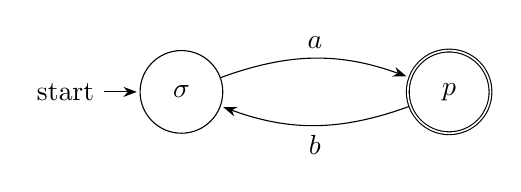
\begin{tikzpicture}[
  >=Stealth,
  shorten >=1pt,
  node distance=3.4cm,
  on grid,
  auto,
  every state/.style={minimum size=1.05cm}
]
  % Trim restriction: the two useful states sigma and p.
  \node[state,initial] (sigma) {$\sigma$};
  \node[state,accepting,right=of sigma] (p) {$p$};

  \path[->]
    (sigma) edge[bend left=20] node {$a$} (p)
    (p) edge[bend left=20] node {$b$} (sigma);
\end{tikzpicture}
\end{document}
